
\chapter{Sistemas HAR }

\label{chap4:sistemas-de-reconocimiento}

\section{Introducción}

\label{sec41:introduccion}El diseño de sistemas con conocimiento
del contexto promueven una interacción novedosa con los usuarios y
diversas aplicaciones en las áreas de ambientes inteligentes, repuesta
a emergencias, vigilancia y otros \cite{Choudhury2008}. Un sistema
con la capacidad de reconocer las actividades humanas por medio del
uso de sensores empotrados posee mecanismos para crear aplicaciones
de cuidado personal, salud y asistencia inteligente. El requerimiento
primordial de un sistema con una aplicación de contexto es que este
pueda ser portado continuamente como atuendo de sus usuarios (un sistema
\abbr{Wearable}). Por lo tanto, un sistema que acompaña continuamente
al usuario puede interaccionar oportunamente con el mismo ya que este
tiene la capacidad de observar en tiempo real las acciones de su portador.
La ventaja adicional de un sistema de este tipo es que puede ser desactivado
fácilmente o removido de la actividad diaria de su usuario.

En este capítulo se definen los componentes principales de un sistema
de reconocimiento de actividades humanas (sistemas \abbr{HAR}). El
objetivo principal del sistema \abbr{HAR} en conjunto es proveer
módulo base para aplicaciones novedosas de contexto. El módulo debe
ser capaz de reconocer varias actividades realizadas rutinariamente
de diferentes maneras, por diferentes usuarios y en diferentes condiciones
contextuales. Las funciones principales de los componentes descritos
en la primera sección exponen los mecanismos para implementar los
mismos en base trabajos relacionados de \abbr{HAR} \cite{Choudhury2008,ReyesOrtiz2015}. 

La última sección cita los requisitos no funcionales para lograr una
aplicación de contexto móvil y ubicua con características especiales
esperadas para este tipo de solución.

\section{Componentes}

\label{sec42:componentes}El diseño de la arquitectura de componentes
de un sistema \abbr{HAR} se rige de acuerdo a las guías de implementación
de una aplicación de aprendizaje automático (\abbr{ML}). De acuerdo
al proceso definido en la sección \ref{sec262:proceso-har}, se tiene
en cuenta la misma estructura de componentes y las mismas fases de
procesamiento de información. Además, se debe contemplar que el proceso
se divide en dos etapas: la etapa de entrenamiento y la de evaluación
\cite{LaraLabrador2013}. 

Ambas etapas requieren la implementación de los mismos componentes,
pero un sistema \abbr{HAR} práctico debe contemplar principalmente
la fase de evaluación, ya que el reconocimiento de actividades resulta
de una predicción basado en un modelo de \abbr{ML} en linea (\emph{On-line
learning}). Sin embargo, la etapa de entrenamiento es un elemento
clave para el sistema ya que es el punto de partida para el aprendizaje
utilizando algoritmos de \abbr{ML} y usualmente se realiza según
sea necesario (\emph{Off-line learning}).

Bajo el marco teórico de los sistemas \abbr{HAR} basados en \abbr{ML},
se han identificado unos componentes comunes para realizar las funcionalidades
de aprendizaje y predicción según \cite{Choudhury2008}. Un sistema
de reconocimiento de actividades posee tres componentes:
\begin{itemize}
\item un \emph{recolector }de medidas
\item un\emph{ procesador }de muestras 
\item un \emph{clasificador }de actividades
\end{itemize}
En la \figref{fig4:componentes-har} se muestra una vista general
de los componentes y sus interrelaciones. Las funcionalidades de cada
componente se describen a continuación. 

\begin{figure}[!tbph]
\centering{}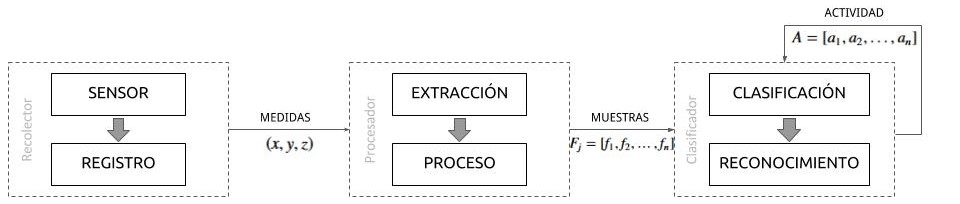
\includegraphics[width=1\columnwidth,width=1\linewidth]{capitulo-4/graphics/diagrama_4_1}\caption[Componentes \abbr{HAR}]{\label{fig4:componentes-har}Componentes de los sistemas \abbr{HAR}}
\end{figure}


\section{Recolector de medidas}

\label{sec43:recolector-datos}El primer paso en el proceso de reconocimiento
primeramente consiste en recolectar medidas de señales obtenidas de
los sensores que observan continuamente a los usuarios. Además, se
procede a realizar un registro de manera organizada e indexada con
respecto al tiempo. Para capturar los datos se requieren instrumentos
de medición apropiados como los sensores (véase \ref{sec23:sensores}).
Los sensores capturan las señales directamente de los usuarios por
medio de observaciones continuas, al estar anexados al cuerpo; en
la cintura, la muñeca, el pectoral, los muslos o en la cabeza \cite{Bao2004}.
También, los sensores podrían ser portados por el usuario ya están
comúnmente empotrados en dispositivos de uso regular como los teléfonos
móviles modernos, en relojes o lentes inteligentes \cite{LaraLabrador2012,Choudhury2008}.

A continuación se describe el método común de registro y organización
de los datos obtenidos de las señales continuas, además de algunos
ejemplos de variables relevantes utilizadas.

\subsection{Registro}

El método de registro consiste en capturar las señales de un sensor
y separar las medidas en una o más variables dependiendo del tipo
de sensor. La organización de los registros se realiza con respecto
al tiempo. Es decir, se dispone de un flujo continuo de datos con
una marca de tiempo almacenados de manera secuencial en un medio permanente
para su posterior procesamiento. 

La marca de tiempo usualmente se mide \emph{mili}-segundos y dependiendo
del sensor el intervalo entre medidas puede variar en el mismo orden,
Ej. con tasa de salida de \texttt{60 \abbr{Hz} }se tendrían 60 medidas
en un segundo. Las señales de sensores pueden clasificarse de la misma
manera que los grupos citados en la sección \ref{sec23:sensores},
según movimiento, posición, ambiente y fisiológicas. 

A continuación se describen dos grupos de señales capturadas por medio
de un sensor específico.

\subsection{Señales Principales}

\subsubsection{Señales de Movimiento}

Los sensores de movimiento proveen señales altamente informativos
para \abbr{HAR} debido a que miden las fuerzas de aceleración y rotación
en tres ejes cuando son portados por sus usuarios. En esta categoría
de sensores se encuentran los acelerómetros y giroscopios. 

Los acelerómetros miden señales de acuerdo a diferentes tipos de movimientos,
incluyendo la aceleración lineal y centrípeta, la gravedad y vibración
en dos o tres dimensiones \cite{Goehl2007}. Las variables medidas
están expresadas en la magnitud de la aceleración ejercida sobre el
dispositivo con respecto la orientación del mismo (Ej. en reposo mide
$-9.8\,m\,s^{-2}$ en dirección al suelo). La señal de la aceleración
dada por $a(t)$ es un vector con respecto al tiempo con tres componentes
en cada eje $(x,y,z)$, cada uno representa una medida $a_{x}$, $a_{y}$
y $a_{z}$. En la \figref{fig4:muestra-ac} se despliegan las medidas
obtenidas por la señal $a(t)$ durante una actividad física determinada.

\begin{figure}[!tbph]
\begin{centering}
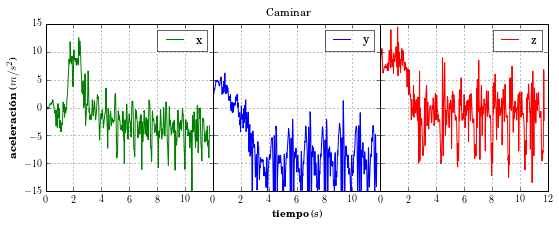
\includegraphics[width=1\columnwidth]{capitulo-4/graphics/signal_a3d}
\par\end{centering}
\caption[Señal de aceleración]{\label{fig4:muestra-ac}Señal de aceleración en tres dimensiones.
Los colores corresponden a los ejes de coordenadas representadas en
la siguiente figura.}
\end{figure}

Los giroscopios, o sensores de razón angular, miden señales de la
rapidez de rotación de los objetos en tres dimensiones \cite{Goehl2007}.
Las variables medidas están expresadas en velocidad angular de rotación
del dispositivo con respecto a los ejes de orientación del mismo (Ej.
en movimiento mide \foreignlanguage{english}{$-0.1\,rad\,s^{-1}$}
en relación a un eje fijo). La señal de la velocidad angular dada
por $w(t)$ es un vector con respecto al tiempo con tres componentes
en cada eje $(x,y,z)$, cada uno representa una medida $w_{x}$, $w_{y}$
y $w_{z}$. La orientación de los ejes con respecto al dispositivo
de medición depende del fabricante del mismo. Los teléfonos móviles
modernos poseen la orientación de los ejes de acuerdo a la siguiente
\figref{fig4:axis-phone}.

\begin{figure}[!tbph]
\begin{centering}
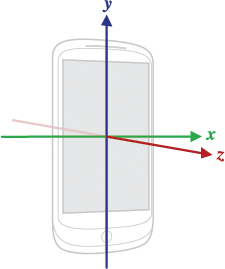
\includegraphics[scale=0.7]{capitulo-4/graphics/axis_device}
\par\end{centering}
\caption[Sistemas de coordenadas relativo a dispositivo]{\label{fig4:axis-phone}Ejes de coordenadas relativas a un teléfono
móvil moderno.}

\end{figure}

Las medidas obtenidas son variaciones con respecto a estos tres ejes
donde el valor $0$ está ubicado en el centro del dispositivo. Las
ventajas de los sensores de movimiento es su amplio uso al reconocer
actividades ambulatorias, como los citados en \cite{Bao2004,Kwapisz2011,ReyesOrtiz2015}.
Los acelerómetros y giroscopios poseen un bajo costo de fabricación,
bajo consumo de energía, y además están incluidos comúnmente en los
teléfonos móviles modernos \cite{Google2016s} debido a su utilidad
en mejorar la interacción humano-máquina por medio de gestos. Varios
trabajos publicados evidencian una alta precisión en \abbr{HAR} utilizando
al menos uno de estos sensores \cite{Bao2004,LaraLabrador2012}.

\subsubsection{Señales de Posición}

Los sensores de posición proveen señales con información adicional
que pueden ser utilizados para efectuar \abbr{HAR} y aplicaciones
de contexto con servicios basados en localización. En esta categoría
están los sensores de orientación (o brújula), magnetómetros y \abbr{GPS}
\cite{Google2016s}.

Las señales del \abbr{GPS} permiten acceder a las coordenadas geográficas
globales como el modo de transporte de un individuo, de acuerdo a
la velocidad estimada. Los teléfonos móviles modernos están equipados
con sensores para captar señales del sistema \abbr{GPS} y también
se puede estimar con buena precisión las coordenadas utilizando una
red celular \abbr{GSM}/\abbr{GPRS} y redes \abbr{WIFI} de corto
alcance. 

La señal de localización utiliza dos variables, conocidas como latitud
y longitud, y son medidas en la unidad radian (Ej. latitud $-57.2322\,rad$
y longitud $-25.3442\,rad$). Los valores de latitud y longitud son
coordenadas del \abbr{WGS} cuyos valores globales oscilan entre -180
a 180 en longitud, y -90 a 90 en latitud.

En la \figref{fig4:gps} se muestra una aplicación móvil para \abbr{Android}
que obtiene la estimación de coordenadas globales al triangular satélites
del \abbr{GPS}. 

\begin{figure}[!tbph]
\begin{centering}
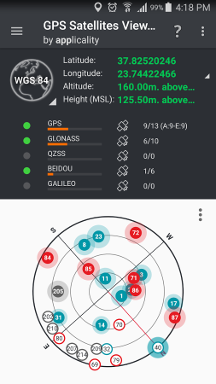
\includegraphics[scale=0.8]{capitulo-4/graphics/gps}
\par\end{centering}
\caption[Coordenadas por \abbr{GPS}.]{\label{fig4:gps}Visualización de satélites y coordenadas globales
basada en \abbr{GPS}.}
\end{figure}

Sin embargo, los \abbr{GPS} tienen cobertura limitada por la dificultad
de obtener señal dentro de edificaciones, o si no está disponible
servicio de red celular o \abbr{WIFI}. También el alto consumo de
energía es un factor importante si las aplicaciones rastrean la localización
en tiempo real. Además, la ubicación de un individuo es particularmente
información sensible para la mayoría de los usuarios y se debe tener
especial atención a no comprometer la privacidad de los datos y tener
el consentimiento del usuario para que este pueda ser rastreado \cite{LaraLabrador2013}.

\subsection{Señales Complementarias}

\subsubsection{Señales del Ambiente}

Los sensores de ambiente solos no proveen información suficiente ya
que los individuos pueden realizar las actividades bajo diversas circunstancias
contextuales en términos de clima, ruido o iluminación. Por lo tanto
estos sensores pueden utilizarse de manera complementaria para detectar
sugestiones adicionales, Ej. el usuario está en el exterior de acuerdo
a la luminosidad, o se encuentra descansando debido a un nivel de
sonido y luminosidad baja \cite{LaraLabrador2013}.

Los sensores de ambiente miden varios atributos del entorno que rodea
al usuario. Algunas señales como la temperatura del aire, presión
atmosférica, iluminación, humedad, y el ruido pueden proveer información
de utilidad para conocer mejor el habitad particular de un usuario.
En esta categoría están los barómetros, fotómetros, termómetros y
micrófonos.

\subsubsection{Señales de Fisionomía}

Los sensores fisiológicos proveen señales de signos vitales de un
individuo. La información sobre el ritmo cardíaco, tasa de respiración
y temperatura del cuerpo podrían ser combinados para enriquecer el
contexto durante el reconocimiento en ciertas aplicaciones específicas
como las orientadas a la salud \cite{LaraLabrador2013}.

\section{Procesador de muestras}

\label{sec44:proceso-se=0000F1ales}El siguiente paso en el reconocimiento
de actividades consiste en procesar las señales obtenidas por sensores
y extraer características relevantes de los datos en bruto. El modelo
de reconocimiento se construye a partir de un conjunto de muestras
etiquetadas utilizando métodos de aprendizaje automático en la etapa
de entrenamiento. Durante la etapa de evaluación las entradas con
las que un modelo construido opera son muestras no clasificadas pero
generadas con la misma técnica de muestreo utilizada durante el entrenamiento.

El procesador de muestras depende en tres tareas bien diferenciadas
que se realizan automáticamente en ambas etapas del proceso de reconocimiento,
adicionalmente se realiza una tarea manual durante la etapa de entrenamiento
llamada etiquetado. A continuación se detallan cada tarea.

\subsection{Etiquetado}

\label{ssec44:labeling}El proceso de aprendizaje automático requiere
de una cantidad moderada de datos recolectados a partir de usuarios
mientras realizan actividades humanas objetivas a nuestro estudio.
Estos datos deben ser recolectadas y etiquetados utilizando un teléfono
móvil inteligente con una aplicación diseñada para el caso, Ej. Utilizando
un teléfono con \abbr{Android} y la aplicación \emph{SensorLog} \cite{SLog2016}. 

El protocolo de recolección consiste en alistar un grupo de personas
que porten un teléfono inteligente mientras realizan con conjunto
específico de actividades y registrar datos por medio de la aplicación.
Las actividades de interés descritas en la sección \ref{sec263:actividades-humanas}
deben ser realizadas portando el teléfono en el bolsillo donde cada
individuo realiza una sesión de caminata, trote, bicicleta o conducir
un vehículo por un periodo de tiempo de 10 a 15 minutos. La recolección
de datos llevada a cabo por medio de la aplicación disponible para
la plataforma \abbr{Android} es mostrada en la \figref{fig4:sensor-log}. 

\begin{figure}[!tbph]
\begin{centering}
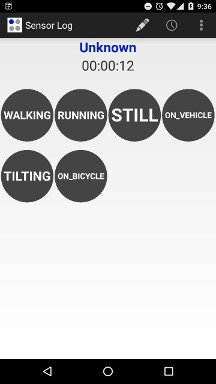
\includegraphics[scale=0.8]{capitulo-4/graphics/sensorlog1}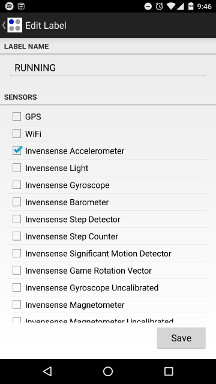
\includegraphics[scale=0.8]{capitulo-4/graphics/sensorlog2}
\par\end{centering}
\caption[Aplicación de recolección \emph{SensorLog}]{\label{fig4:sensor-log}Aplicación de recolección \emph{SensorLog
}con interfaces de usuario para configurar y controlar la sesión de
entrenamiento}
\end{figure}

Así como se ve en la figura, la aplicación tiene una interfaz de usuario
simple que permite elegir los sensores de donde recolectar datos (Ej.
\abbr{GPS}, acelerómetro, giroscopio) para la sesión, las acciones
de iniciar y parar la actividad, y las etiquetas de la actividad que
el usuario realiza durante el entrenamiento. Las etiquetas utilizadas
en el proceso de recolección son:
\begin{itemize}
\item Caminar
\item Trotar
\item Quieto\footnote{A pesar de que esta actividad no representa un movimiento se incluye
como parte del estudio}
\item En bicicleta
\item En vehículo
\item \emph{Girando}\footnote{Esta no es una actividad física sino un comportamiento errático de
la orientación del teléfono}
\end{itemize}
La recolección se realiza obteniendo medidas a una razón de 60 a 100
milisegundos por lo que se registran aproximadamente 60 a 100 muestras
por segundo. Para asegurar la calidad de la recolección inicial de
datos las primeras sesiones de entrenamiento son supervisadas para
preparar las condiciones adecuadas del entrenamiento físico a elección
del participante.

\subsection{Filtro de Señal}

\label{ssec44:filtering}Teóricamente, si un dispositivo equipado
con sensores de movimiento está en reposo la señal de aceleración
$a(t)$ mediría cero (0) en dos ejes. Por ejemplo, en los ejes $x$
e $y$ no habría registro de medidas distintas a cero (0), y el eje
$z$mediría en dirección al suelo $-9.8\,m\,s^{-2}$. Sin embargo,
los sensores electrónicos pueden introducir cierta inestabilidad en
la señal (conocida como \emph{jitter}) provocando una fluctuación
en las lecturas debido a errores en la medición afectando la calidad
de los datos. Por lo tanto, a pesar de que un dispositivo con sensor
de movimiento esté completamente quieto en la mesa, las lecturas podrían
registrar ruido en los datos, Ej. errores del orden de $\pm0.005$. 

Entonces, para reducir ruido de la señal se debe aplicar uno o más
filtros. El filtro permite suavizar la señal por medio de una función
simple como la del cálculo de promedios variables\footnote{\emph{moving average}}
o por un método como el de \emph{Butterworth} \cite{ReyesOrtiz2015}. 

Para el análisis de este trabajo se utilizó el filtro de señal de
promedios variables debido a su simplicidad y aplicabilidad basado
en otros trabajos como \cite{Yang2009}. El filtro de señal se puede
definir con la siguiente función $M$ descrita a continuación:

\label{def4:moving-average}\newtheorem{defs}{Definición}

\begin{defs}(\emph{Moving average}) Dada una secuencia $\left\{ a_{i}\right\} _{i=1}^{N}$,
un $n$-\emph{moving average} es una nueva secuencia $\left\{ s_{i}\right\} _{i=1}^{N-n+1}$
definida a partir de $a_{i}$ tomando la media aritmética de las \emph{sub}-secuencias
de tamaño $n$ donde,

\begin{eqnarray}
s_{i} & = & \frac{1}{n}\sum_{j=i}^{i+n-1}a_{j}
\end{eqnarray}

Así que las secuencias $S_{n}$ dado los $n$-\emph{moving averages}
serian 

\begin{eqnarray}
S_{2} & = & \frac{1}{2}(a_{1}+a_{2},a_{2}+a_{3},...,a_{n-1}+a_{n})
\end{eqnarray}

\begin{equation}
S_{3}=\frac{1}{3}(a_{1}+a_{2}+a_{3},a_{2}+a_{3}+a_{4},...,a_{n-2}+a_{n-1}+a_{n})
\end{equation}

y así sucesivamente.\end{defs}

Como ejemplo, en la \figref{fig4:filter-maf} se despliegan las gráficas
de una señal de aceleración $a_{y}$ para la dimensión $y$ y su correspondiente
señal filtrada con la función $M(a_{y})$ construida a partir de una
secuencia $S_{5}$ durante un intervalo de $1.6$ segundos. Como se
puede apreciar, la señal resultante está ligeramente suavizada debido
al filtrado de valores extremos resultado de perturbaciones bruscas
o ruido en la señal.

\begin{figure}[!tbph]
\begin{centering}
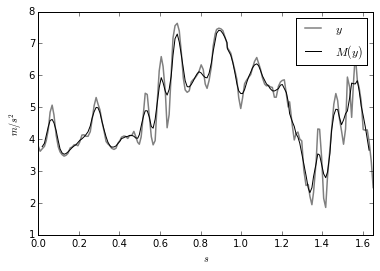
\includegraphics{capitulo-4/graphics/moving_average}
\par\end{centering}
\caption[Señal filtrada por la función $M$]{\label{fig4:filter-maf}Señal filtrada por promedios variables.}
\end{figure}


\subsection{Muestreo}

\label{ssec44:sampling}La realización de actividades humanas son
efectuadas durante periodos de tiempo de larga duración, en el orden
de los segundos o minutos. Esta taza es mucho mayor comparado con
las tazas de muestreos de los sensores, las cuales pueden llegar hasta
\texttt{250 \abbr{Hz}} (o \texttt{250} muestras por segundo). Una
simple medida capturada en un instante (Ej. la aceleración de $-2.5\,m\,s^{-2}$
en el eje $y$) no provee suficiente información para describir qué
actividad está llevando acabo un persona. Por lo tanto, las actividades
humanas deben ser reconocidas a partir de muestras extraídas en ventanas
de tiempo $w$ en vez de utilizar una sola medida instantánea en $t$. 

En la \tabref{tab4:ex-signal} se muestra una tabla con posibles medidas
instantáneas para la señal de aceleración $a(t)$ en una ventana de
tiempo $w_{j}$ con una taza de muestreo $r$asociada al sensor.

\begin{table}[!tbph]
\begin{centering}
\begin{tabular}{|c|c|c|c|c|}
\hline 
$w$ & $t$ & $a_{x}$ & $a_{y}$ & $a_{z}$\tabularnewline
\hline 
\hline 
$j$ & $0$ & \texttt{$1.3$} & \texttt{$-2.1$} & \texttt{$0$}\tabularnewline
\hline 
$j$ & $1/r$ & \texttt{$1.4$} & \texttt{$-2.3$} & \texttt{$0.1$}\tabularnewline
\hline 
$j$ & $2/r$ & \texttt{$1.1$} & \texttt{$-2.6$} & \texttt{$0$}\tabularnewline
\hline 
$j$ & $\ldots$ & \texttt{$\ldots$} & \texttt{$\ldots$} & \texttt{$\ldots$}\tabularnewline
\hline 
$j$ & $t_{max}$ & \texttt{$1.8$} & \texttt{$2.2$} & \texttt{$-0.4$}\tabularnewline
\hline 
\end{tabular}
\par\end{centering}
\caption[Medidas instantáneas de aceleración ]{\label{tab4:ex-signal}Ejemplo de medidas instantáneas de aceleración
en una ventana de tiempo.}
\end{table}

Las ventanas de tiempo hacen que las señales queden segmentadas en
muestras discretas utilizadas como unidades de reconocimiento de actividad.
De esta manera, cada ventana tiene inequívocamente una actividad humana
asociada y de esta manera podemos satisfacer el requisito planteado
por la definición del problema \ref{def2:harp-rel} en la sección
\ref{sec261:definicion-har}. 

Para incrementar la cantidad de muestras se utiliza una superposición
de $50\%$ con ventanas consecutivas y con tamaño de $2.56$ segundos,
como es recomendado por otros trabajos con técnicas de reconocimiento
\cite{Bao2004,ReyesOrtiz2015}. La superposición evita que ciertos
eventos se pierdan y las actividades se trunquen. La elección de este
tamaño de ventana produce muestras con medidas de tamaño fijo calculadas
aproximadamente con la ecuación \ref{eq4:window-size}. Este tamaño
es bastante conveniente por razones halladas en \cite{ReyesOrtiz2015}.

\begin{equation}
2.56\,\mathrm{sec}\times50\mathrm{\,Hz}=128\,\mathrm{medidas}\label{eq4:window-size}
\end{equation}

Cada muestra debe ser transformada en vectores característicos al
pasar por un proceso de extracción de valores que se describen en
la siguiente sección.

\subsection{Extracción}

\label{ssec44:extraction}Rememorando la definición del problema relajado\ref{def2:harp-rel}
en la sección \ref{sec261:definicion-har}, la incógnita principal
consiste en la comparación de las muestras provenientes de dos ventanas
$w_{1}$ y $w_{2}$, cada muestra con medidas $S_{j}$ que corresponden
a señales completamente distintas. Estas señales no serán idénticas
por más que sean obtenidas del mismo individuo realizando la misma
actividad física. Por lo tanto, para comparar muestras entres sí es
necesario extraer valores característicos en cada ventana $w_{j}$
por medio del filtro de información relevante y el calculo de valores
que identifiquen de cierta manera a las señales. 

El proceso de extracción se traduce en vectores característicos (\abbr{feature vectors})
con información relevante que componen varias métricas calculadas
en base a las ventanas $w_{j}$ en el dominio del tiempo. Las ventanas
son transformadas en el dominio de la frecuencia con métodos discretos
de\emph{ Fourier} utilizando algoritmos \abbr{FFT} con números reales. 

Los métodos de cálculo pueden ser de tipos estadísticos y estructurales
\cite{LaraLabrador2013} en base a lo propuesto por otros trabajos
precedentes como\cite{Yang2009,Bao2004}. Las métricas estadísticas
con respecto al tiempo y frecuencia utilizadas en este trabajo son:
\begin{enumerate}
\item \textbf{Media aritmética}: medida de tendencia central en la señal.
\item \textbf{Valor máximo}: medida de valor extremo en la señal.
\item \textbf{Valor mínimo}: medida de valor extremo en la señal.
\item \textbf{Desviación estándar}: media de dispersión en la señal.
\item \textbf{Energía}: promedio de suma de los cuadrados en la señal.
\item \textbf{Entropía}: (de Shannon) medida de incertidumbre utilizada
comúnmente en la Teoría de la Información aplicada a la señal en el
dominio de la frecuencia. Estima la cantidad de información en la
señal.
\item \textbf{Asimetría:} medida de distribución de simetría en el dominio
de la frecuencia.
\item \textbf{Curtosis:} medida de distribución de concentración en el dominio
de la frecuencia.
\item \textbf{Rango intercuartíl:} medida de dispersión de la diferencia
entre el tercer y primer cuartíl.
\item \textbf{Coeficientes autorregresivos:} los coeficientes obtenidos
utilizando el método de Burg que aplica un modelo autorregresivo para
encajar en la señal. La operación es aplicada a la señal en el dominio
del tiempo y produce cuatro (4) valores correspondientes al algoritmo
de 4to orden.
\item \textbf{Promedio en frecuencia:}medida de tendencia central en el
dominio de la frecuencia.
\end{enumerate}
En la \tabref{tab4:metricas} se resumen las métricas enumeradas anteriormente
en el orden establecido junto con el nombre de función y la formulación
matemática correspondiente para una señal dada$s$ en cualquier ventana$w_{j}$
de tamaño$n$.

\begin{table}[!tbph]
\begin{centering}
\begin{tabular}{|l|l|}
\hline 
Función & Formulación\tabularnewline
\hline 
\hline 
\texttt{mean(s)} & $\overline{s}=\frac{1}{n}\sum_{i=1}^{n}s_{i}$\tabularnewline
\hline 
\texttt{std(s)} & $\sigma=\sqrt{\frac{1}{n}\sum_{i=1}^{n}\left(s_{i}-\overline{s}\right)}$\tabularnewline
\hline 
\texttt{max(s)} & $\mathrm{max}(s)$\tabularnewline
\hline 
\texttt{min(s)} & $\mathrm{min}(s)$\tabularnewline
\hline 
\texttt{skewness(s)} & $\mathrm{E}\left[\left(\frac{s-\overline{s}}{\sigma}\right)^{3}\right]$\tabularnewline
\hline 
\texttt{kurtosis(s)} & $\frac{\mathrm{E}\left[\left(s-\overline{s}\right)^{4}\right]}{\mathrm{E}\left[\left(s-\overline{s}\right)^{2}\right]^{2}}$\tabularnewline
\hline 
\texttt{energy(s)} & $\frac{1}{n}\sum_{i=1}^{n}s_{i}^{2}$\tabularnewline
\hline 
\texttt{entropy(s)} & $s_{s}c_{i}=\sum_{i=1}^{n}c_{i}\log\left(c_{i}\right)\mathrm{\mathtt{\mathrm{,}}\,c_{i}}=s_{i}/\sum_{j=1}^{n}s_{j}$\tabularnewline
\hline 
\texttt{irq(s)} & $Q3(s)-Q1(s)$\tabularnewline
\hline 
\texttt{autoregression(s)} & $ar=\mathrm{arburg}\left(s,4\right)\mathrm{,}\,ar\in\mathbb{R}^{4}$\tabularnewline
\hline 
\texttt{meanFreq(s)} & $\sum_{i=1}^{n}\left(is_{i}\right)/\sum_{j=1}^{n}s_{j}$\tabularnewline
\hline 
\end{tabular}
\par\end{centering}
\caption[Métricas de valores característicos]{\label{tab4:metricas}Métricas para el calculo de vectores característicos
según\cite{ReyesOrtiz2015}.}
\end{table}

Las señales procesadas del conjunto $S$ corresponden al atributo
de la aceleración. Se utiliza un conjunto$S=\left\{ s_{0}\right\} $
con $k=1$, donde $s_{0}$ corresponde a la magnitud del vector resultante
de las medidas de fuerza ejercida en los tres ejes según la ecuación\ref{eq4:magnitud}.

\begin{equation}
\lVert a\rVert=\sqrt{a_{x}^{2}+a_{y}^{2}+a_{z}^{2}}\label{eq4:magnitud}
\end{equation}

Se eligió utilizar la magnitud $\lVert a\rVert$ del vector excluyendo
los valores unitarios en cada dimensión $a_{x}$,$a_{y}$,$a_{z}$
por los siguientes motivos:
\begin{itemize}
\item Simplicidad para utilizar la técnica de \abbr{DT}.
\item Para cancelar el efecto de variaciones en la orientación del teléfono
\cite{Schneider2014}.
\item Reducir la dimensión de características (a un tercio) evitando sobreajustes\footnote{\emph{overfitting}}.
\end{itemize}
El proceso de extracción transforma una ventana $w_{j}$ con señales
originales en un vector característico $F_{j}$ de dimensión $p$
como es representado en el ejemplo de la \tabref{tab4:features}.
Cada valor $\mathrm{f}_{0},\mathrm{f}_{1},\ldots,\mathrm{f}_{p}$
donde$p=14$ son obtenidos con una métrica particular enumerada anteriormente.

\begin{table}[!tbph]
\begin{centering}
\begin{tabular}{|c|c|c|c|}
\hline 
$w$ & $\mathrm{f}_{0}$ & $\ldots$ & $\mathrm{f}_{p}$\tabularnewline
\hline 
\hline 
$0$ & $2.71$ & \texttt{$\ldots$} & \texttt{$-2.30$}\tabularnewline
\hline 
$\ldots$ & $\ldots$ & \texttt{$\ldots$} & \texttt{$\ldots$}\tabularnewline
\hline 
$j$ & $2.91$ & \texttt{$\ldots$} & \texttt{$-4.11$}\tabularnewline
\hline 
$\ldots$ & $\ldots$ & \texttt{$\ldots$} & \texttt{$\ldots$}\tabularnewline
\hline 
$m-1$ & $2.56$ & \texttt{$\ldots$} & \texttt{$-5.56$}\tabularnewline
\hline 
\end{tabular}
\par\end{centering}
\caption[Métricas de proceso de extracción]{\label{tab4:features}Métricas procesadas a partir de las medidas
de señales}
\end{table}

Por último, se considera que tanto $S_{j}$ como $F_{j\ensuremath{}}$
tienen relación con al menos una etiqueta $\mathrm{a}_{k}$ particular
del conjunto $A$ ya sea debido a la función $f(S_{j})$ como resultado
de una evaluación, o como información en los datos del conjunto entrenamiento.

\section{Clasificador de actividades }

\label{sec45:clasificador}Un sistema \abbr{HAR} es similar a cualquier
aplicación de aprendizaje automático (\abbr{ML}) donde se requiere
de un algoritmo diseñado para extraer información desde los datos.
En este contexto los patrones son descubiertos a partir de un conjunto
de observaciones denominadas instancias \cite{LaraLabrador2013}.
El propósito principal del algoritmo es de clasificar los datos desconocidos.
Rememorando el \ref{chap:Aprendizaje-Automatico}, la entrada aplicada
a un algoritmo de \abbr{ML} es un conjunto de entrenamiento\footnote{\emph{training set}}
y el resultado del mismo es un clasificador\footnote{\emph{classifier}}
\cite{Rajaraman2011}. En la \figref{fig4:clasificador} se muestra
una gráfico esquemático adaptado al problema \abbr{HAR} del proceso
de extracción de conocimiento con algoritmos de aprendizaje automático
\cite{Raschka2014}.

\begin{figure}[H]
\begin{centering}
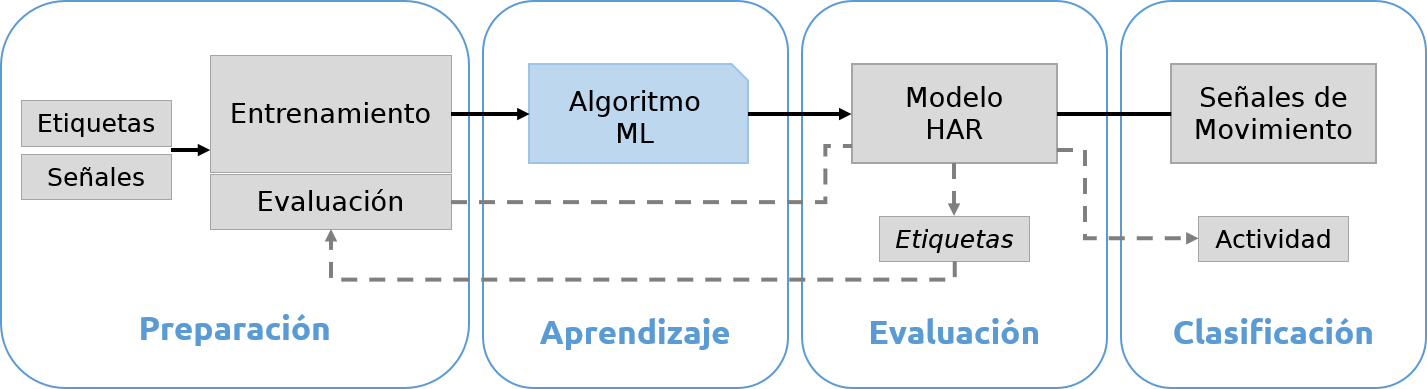
\includegraphics[width=1\columnwidth]{capitulo-4/graphics/clasificacion}
\par\end{centering}
\caption[Modelo de aprendizaje automático]{\label{fig4:clasificador}Construcción de modelo \abbr{HAR} basado
en técnicas de aprendizaje automático.}
\end{figure}

En esta sección se detallan los pasos del proceso común de aprendizaje
automático.

\subsection{Preparación}

Es parte esencial de todo algoritmo de aprendizaje automático supervisado
contar con un conjunto de instancias de entrenamiento y la información
adicional de clasificación. Durante las secciones precedentes se abarcaron
las tareas de preparación de los datos utilizados en el entrenamiento
y la clasificación. Las preparación se compone de varias tareas que
inciden en la mejora del clasificador resultante, las cuales se listan
a continuación:
\begin{itemize}
\item Limpieza y formateo de datos
\item Extracción de vectores característicos
\item Omitir instancias duplicadas o altamente correlativas
\item Reducir la cantidad de instancias de entrada
\item Normalizar el domino de los datos de las instancias
\item Separar las instancias de entrada: en conjunto de entrenamiento y
evaluación
\end{itemize}
Cada instancia es un vector característico $F_{j}$ calculado a partir
de las señales $s$ contenidas en una ventana de tiempo $w_{j}$.
Todo clasificador supervisado requiere de un conjunto de entrenamiento
etiquetado con la información de clasificación conocida, así como
se muestra en la \tabref{tab4:labeled}. 

\begin{table}[!tbph]
\begin{centering}
\begin{tabular}{|c|c|c|c|c|}
\hline 
$w$ & $\mathrm{f}_{0}$ & $\ldots$ & $\mathrm{f}_{m}$ & \emph{Actividad}\tabularnewline
\hline 
\hline 
$0$ & $2.71$ & \texttt{$\ldots$} & \texttt{$-2.30$} & \texttt{\small{}Desconocido}\tabularnewline
\hline 
$\ldots$ & $\ldots$ & \texttt{$\ldots$} & \texttt{$\ldots$} & \texttt{$\ldots$}\tabularnewline
\hline 
$j$ & $2.91$ & \texttt{$\ldots$} & \texttt{$-2.11$} & \texttt{\small{}Corriendo}\tabularnewline
\hline 
$\ldots$ & $\ldots$ & \texttt{$\ldots$} & \texttt{$\ldots$} & \texttt{$\ldots$}\tabularnewline
\hline 
$k-1$ & $2.56$ & \texttt{$\ldots$} & \texttt{$-2.56$} & \texttt{\small{}Caminando}\tabularnewline
\hline 
\end{tabular}
\par\end{centering}
\caption[Instancias etiquetadas]{\label{tab4:labeled}Conjunto de entrenamiento etiquetado con información
de clasificación.}
\end{table}

La tarea de etiquetado puede ser realizada de manera manual (como
en la sección \ref{ssec44:labeling}), como también de manera automatizada.
El etiquetado de datos detectados a partir de individuos que realizan
diferentes actividades es una tarea relativamente fácil. Algunos sistemas
guardan datos del sensor en medios no volátiles mientras que una persona
del equipo de investigación supervisa el proceso de recolección y
registra de forma manual la etiqueta de actividad en cada intervalo
de tiempo. Otros sistemas se caracterizan por una aplicación móvil
que permite al usuario seleccionar la actividad que se realiza a partir
de una lista, de esta manera, cada muestra se corresponde con una
etiqueta de actividad. Este ultimo enfoque es utilizado en este trabajo.

Es importante considerar las etiquetas asignadas a los datos originales
de la señal en cada ventana de tiempo. Las etiquetas asignadas a los
datos definen la relación $(F_{j},a_{k})$, entre etiquetas y cada
vector característico. 

\subsection{Aprendizaje}

El requisito primordial para la tarea de aprendizaje es escoger al
algoritmo adecuado para la clasificación. Así como se presenta en
el capitulo \ref{chap:Aprendizaje-Automatico} la elección es el algoritmo
C4.5 (\ref{algoC45}) basado en el enfoque de arboles de decisión.
El proceso de aprendizaje puede realizarse en base a tres metodologías
\cite{Rajaraman2011}.

El aprendizaje \emph{basado en lotes} consiste en contar con la mayor
cantidad de datos de entrenamiento al principio del proceso y utilizarlo
íntegramente para construir el modelo una sola vez. Por otro lado
el aprendizaje \emph{en linea} puede contar con los datos de entrenamiento
a medida que se disponen de los mismos, como en un flujo de datos,
estos son examinados una sola vez y no pueden ser revisados. Con este
método se mantiene el modelo constantemente, a medida que nuevas instancias
de entrenamiento son recibidas, se puede elegir modificar el modelo
y mejorarlo con nuevas instancias. 

Las ventajas de realizar el aprendizaje en linea se pueden apreciar
a simple vista. El conjunto de entrenamiento de entrada puede ser
de gran tamaño sin necesidad de acceder a más de una instancia la
vez. También, el modelo puede adaptarse a los cambios que emerjan
en la población de instancias de entrenamiento a medida que transcurre
el tiempo.

Una mejora aplicada al aprendizaje en linea es el aprendizaje \emph{activo}.
El clasificador se construye primeramente utilizando un conjunto de
entrenamiento, pero a la par se pueden recibir datos no clasificados
para que el modelo los clasifique. Si el modelo realiza una clasificación
con mucha incertidumbre, se puede requerir que la instancia sea verificada
para aseverar la clasificación a un costo significativo. 

Por ejemplo, la instancia puede ser retenida y verificada manualmente
por medio de una encuesta en terreno a personas reales. De esta manera
las instancias verificadas pueden luego ser utilizadas para mejorar
el modelo clasificador (véase en la \figref{fig4:componentes-har}
la retroalimentación). 

En este trabajo se busca tener nuevas instancias de entrenamiento
por medio de un proceso colaborativo, partiendo inicialmente de un
conjunto de instancias de entrenamiento e ir mejorando la población
con una encuesta dirigida por medio del uso del sistema \abbr{HAR}.

\subsection{Evaluación}

Uno de los tópicos primordiales de los algoritmos de \abbr{ML} es
la manera en que los datos son tratados al clasificar datos desconocidos
y utilizados para construir un modelo de reconocimiento efectivo.
Al tratar con los datos, es buena estrategia dividir las instancias
de entrada disponibles en un conjunto de entrenamiento y un remanente
conocido como conjunto de validación\emph{}\footnote{\emph{test set}}.
El problema común de los algoritmos de \abbr{ML} es el error asociado
al sobreajuste, es decir, la clasificación resulta como se espera
en el conjunto de entrenamiento pero ante la mínima variación con
datos desconocidos de una población mayor el resultado se torna atípico
o con errores de clasificación \cite{Rajaraman2011}. 

El conjunto de validación permite evaluar el clasificador determinando
si se sobreajustan los resultados y con cuanta precisión es efectivo
el modelo. La precisión es la proporción de instancias correctamente
clasificadas. El sobreajuste es una medida del error en base a la
precisión del modelo con instancias en el conjunto de evaluación.

Evaluar métricas permite realizar ajustes a los parámetros al construir
el algoritmo de aprendizaje automático. Por ejemplo, si se construyen
árboles de decisión, se pueden limitar la cantidad de niveles del
árbol.

\subsection{Clasificación}

TODO:

\section{Capacidades deseables}

\subsection{Características no funcionales}

\label{ssec46:caracteristicas}Existen un conjunto de características
deseables que deben ser satisfechas para la construcción efectiva
de los sistemas de reconocimiento. Estas características abordan cuestiones
de diseño importantes que conciernen a la calidad y al funcionamiento
del sistema. Las características se listan a continuación:
\begin{enumerate}
\item Portabilidad, el sistema utiliza sensores adjuntos a los individuos
(Ej. el acelerómetro) y no deben obstruir las actividades cotidianas
de los usuarios durante su uso. El fin es de evitar que se afecte
la adopción masiva del sistema. 
\item Conectividad, el sistema debe transmitir de manera confiable los datos
recolectados y/o procesados a algún componente desplegado de forma
remota. 
\item Almacenamiento, el sistema debe persistir los datos recolectados y/o
procesados de manera local en el dispositivo móvil con el fin de mantener
la calidad y minimizar la cantidad transferida a otros componentes.
\item Procesamiento, el sistema debe procesar y transformar los datos en
bruto para producir información relevante para el reconocimiento de
actividades.
\item Ubiquidad, el sistema debe operar en cualquier condición y contexto
en que la persona se encuentre sin interferir u obligar al usuario
a interactuar con el sistema.
\item Uso de energía, el sistema debe preservar el uso de energía en los
dispositivos móviles que están implementados. La lectura de datos,
el procesamiento y la conectividad no deben incurrir en gastos excesivos
de energía para que el sistema pueda operar.
\item Privacidad, el sistema debe mantener de manera confidencial los datos
recolectados y/o producidos durante la adopción masiva del sistema,
además de alertar sobre la utilización de datos sensibles que requieran
el consentimiento del usuario.
\end{enumerate}

\section{Conclusión}

En este capítulo se abarcaron los aspectos prácticos en detalle de
los sistemas de reconocimiento de actividades humanas partiendo de
los fundamentos teóricos y las técnicas existentes en la literatura.
Principalmente, se enmarco la estructura del sistema \abbr{HAR} con
sus componentes principales, el proceso general de reconocimiento
y las tareas funcionalidades básicas. Finalmente, se citan algunos
aspectos que tienen que ver con características esperadas en una aplicación
de contexto aplicadas a nuestro problema en particular.
